\subsection{What is R?}
\makesubcontentsslidessec


\begin{frame}
  \begin{block}{What is R?}\pause
  \begin{minipage}{.675\textwidth}
  \begin{itemize}[<+-|alert@+>]
    \item \emph{lingua franca} for data analytics and statistical computing.
    \item Part programming language, part data analysis package.
  \end{itemize}
  \end{minipage}
  \hfill
  \begin{minipage}{.3\textwidth}
    \centering
\includegraphics[scale=.85]{../common/pics/Rlogo}
  \end{minipage}
  \begin{itemize}
    \item Dialect of S (May 5, 1976, Bell Labs).
    \item Free (GPL $\geq 2$)
    \item A C program (mostly): 52\% C, 26\% Fortran, 22\% R
    \item Highly extensible; has over 5000 user-contributed packages.
  \end{itemize}
\end{block}
\end{frame}



\def\Put(#1,#2)#3{\leavevmode\makebox(0,0){\put(#1,#2){#3}}}
\begin{frame}
\vspace{-.1cm}
\begin{block}{Who uses R?}
\ \\[6.5cm]\ 
\end{block}
% top line
\Put(0,400){
\includegraphics[scale=1]{../common/pics/R_using_logos/oracle}}
\Put(135,410){
\includegraphics[scale=.1]{../common/pics/R_using_logos/merck}}
\Put(245,420){
\includegraphics[scale=.12]
  {../common/pics/R_using_logos/kickstarter}}
\Put(260,360){
\includegraphics[scale=.09]
  {../common/pics/R_using_logos/johndeere}}
%%%%
% second line
\Put(-5,315){
\includegraphics[scale=.2]{../common/pics/R_using_logos/boa}}
\Put(87,310){
\includegraphics[scale=.15]{../common/pics/R_using_logos/fb}}
\Put(145,355){
\includegraphics[scale=.12]{../common/pics/R_using_logos/ebay}}
\Put(135,270){
\includegraphics[scale=.9]{../common/pics/R_using_logos/mozilla}}
\Put(177,310){
\includegraphics[scale=.35]{../common/pics/R_using_logos/nyt}}
\Put(247,300){
\includegraphics[scale=.1]{../common/pics/R_using_logos/nist}}
%%%%
% third line
\Put(-50,210){
\includegraphics[scale=.05]{../common/pics/R_using_logos/shell}}
\Put(15,200){
\includegraphics[scale=.17]{../common/pics/R_using_logos/pfizer}}
\Put(92,188){
\includegraphics[scale=.22]{../common/pics/R_using_logos/fda}}
\Put(160,170){
\includegraphics[scale=.08]{../common/pics/R_using_logos/twitter}}
\Put(170,240){
\includegraphics[scale=.1]{../common/pics/R_using_logos/orbitz}}
\Put(250,250){
\includegraphics[scale=.12]{../common/pics/R_using_logos/cfpb}}
\Put(200,210){
\includegraphics[scale=.6]{../common/pics/R_using_logos/novartis}}
\Put(204,160){
\includegraphics[scale=.16]{../common/pics/R_using_logos/lloyds}}
%%%%
% fourth line
\Put(-50,90){
\includegraphics[scale=.12]{../common/pics/R_using_logos/google}}
\Put(50,130){
\includegraphics[scale=.12]{../common/pics/R_using_logos/bing}}
\Put(50,70){
\includegraphics[scale=.29]{../common/pics/R_using_logos/ford}}
\Put(135,80){
\includegraphics[scale=.25]{../common/pics/R_using_logos/zillow}}
\Put(205,80){
\includegraphics[scale=.15]{../common/pics/R_using_logos/okcupid}}
\end{frame}



% \begin{frame}
%   \begin{block}{Language Paradigms}\pause
%   \begin{center}
%     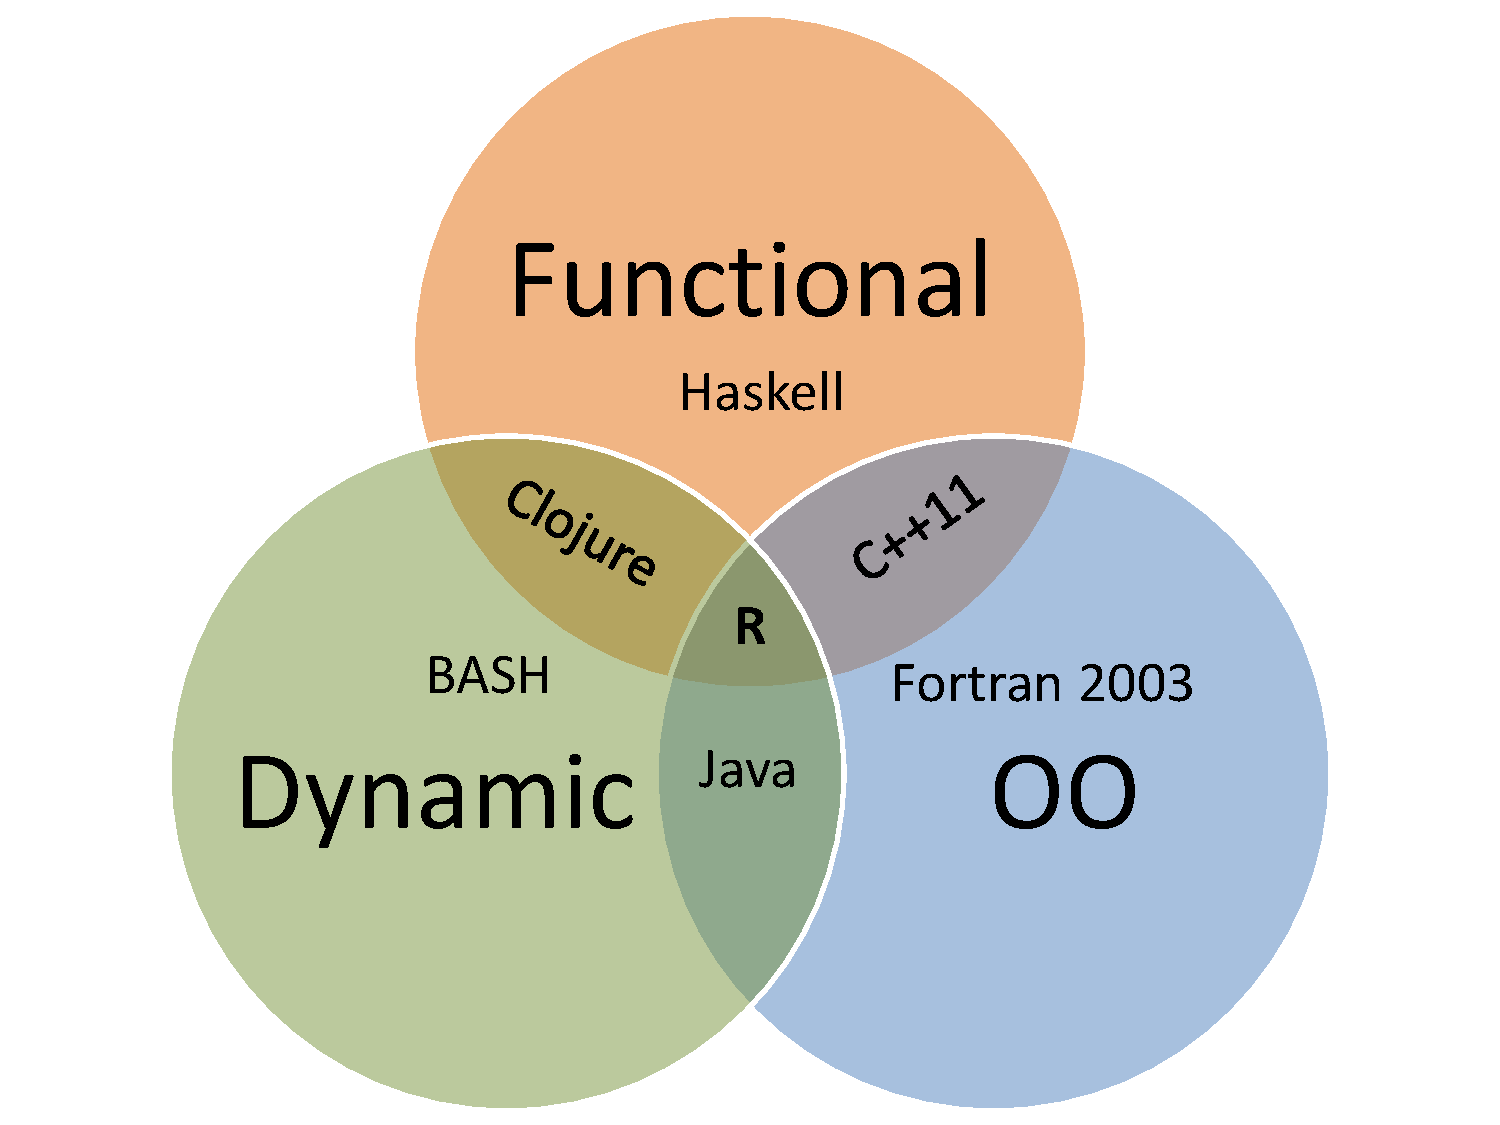
\includegraphics[scale=.35]{../common/pics/languages}
%   \end{center}
%   \end{block}
% \end{frame}



\begin{frame}
\begin{block}{The R Language}\pause
\begin{itemize}
  \item R is slow; if you don't know what you're doing, it's \emph{really} slow.
  \item High-level language.
  \item Syntax designed for data: models are first-class constructs, 
missingness is built into the core of the language, \dots
\end{itemize}
\end{block}
\end{frame}



\begin{frame}
\begin{block}{The R Language}\pause
  If you come from CS, you may find \R a bit strange:
  \begin{itemize}
    \item Storage: logical, int, double, double complex, character (strings)
    \item Structures: vector, matrix, array, list, dataframe
    \item Caveats: (Logical) \code{TRUE}, \code{FALSE}, \code{NA}
    \item In fact, there's an \code{NA} for each type:
    \begin{itemize}
      \item Integer: $-\left(2^{-31}-1\right)$
      \item Double: value at address \code{0x7FF00000000007A2LL}
    \end{itemize}
    \item 3 official OOP systems (none of them work like anything you're used 
to), several unofficial ones.
    \item No official support for C++; several unofficial packages supporting 
C++.
  \end{itemize}
\end{block}
\end{frame}



\begin{frame}{But you can't deny its popularity!}
  \begin{center}
    IEEE Spectrum's 2014 Ranking of Programming Languages\\
    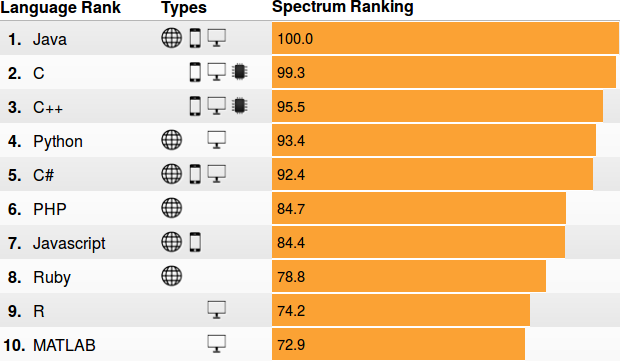
\includegraphics[scale=.6]{../common/pics/ieee_spectrum}
  \end{center}
 {\scriptsize See: 
\url{%
http://spectrum.ieee.org/static/interactive-the-top-programming-languages\#index
}}
\end{frame}




\begin{frame}
  \begin{block}{Resources for Learning R}\pause
  \begin{itemize}[<+-|alert@+>]
    \item \emph{Advanced R} by Hadley Wickham: \url{http://adv-r.had.co.nz/}
    \item \emph{The Art of R Programming} by Norm Matloff:  
\url{http://nostarch.com/artofr.htm}\\[.2cm]

    \item \emph{An Introduction to R} by Venables, Smith, and the R Core Team:
\url{http://cran.r-project.org/doc/manuals/R-intro.pdf}\\[.2cm]

    \item \emph{The R Inferno} by Patrick Burns:
\url{http://www.burns-stat.com/pages/Tutor/R_inferno.pdf}\\[.2cm]

    \item Mathesaurus:  \url{http://mathesaurus.sourceforge.net/}\\[.2cm]

    \item R programming for those coming from other languages:  
\url{http://www.johndcook.com/R_language_for_programmers.html}\\[.2cm]

    \item \emph{aRrgh: a newcomer's (angry) guide to R}, by Tim Smith and Kevin 
Ushey: 
    \url{http://tim-smith.us/arrgh/}
  \end{itemize}
\end{block}
\end{frame}


\begin{frame}
  \begin{block}{Other Invaluable Resources}\pause
  \begin{itemize}[<+-|alert@+>]
    \item \emph{R Installation and Administration}: 
\url{http://cran.r-project.org/doc/manuals/R-admin.html}
    \item \emph{Writing R Extensions}: 
\url{http://cran.r-project.org/doc/manuals/R-exts.html}
     \item Mailing list archives: \url{http://tolstoy.newcastle.edu.au/R/}
     \item The \code{[R]} stackoverflow tag.
  \end{itemize}
\end{block}
\end{frame}